% ------------------------------------------------------------------------------------------------------------------------------------------------
\chapter{Cluster scaling and performance analysis}
\label{chap:perf-scalability}

This section will focus on analysing as well as presenting improvements to the cluster deployment which can and have been applied to the Hadoop cluster leveraged by the Analyser application presented in previous chapters.

In Section \ref{sec:scaling-hadoop} several challanges and typical problems with scaling Hadoop clusters will be presented, and then followed up by solutions applied during the work on this thesis.

Section \ref{sec:scaling-akka} will briefly explain scalability concerns related to an Akka based cluster deployment, yet as this component has not been as critical to overal system performance as the Analyser and Hadoop cluster, the Akka cluster has been deemed ''good enough'' for the scope of this paper.

\todo{explain what section does what}

% ------------------------------------------------------------------------------------------------------------------------------------------------
\section{Scaling Hadoop}
\label{sec:scaling-hadoop}
This section will focus on analysing and tuning the various settings of the Hadoop cluster deployed for the previously described Analyser application. Subsections focus on tuning the cluster on a setting--by--setting basis yet the tuning will always be enforced by a business need, which in this case will be represented as the need to speed up processing of the map reduce pipelines producing results which were explained in Chapter \ref{chap:analysis-examples}.

\subsection{Storing images on HDFS, while avoiding the ''Small Files Problem''}
\label{sec:sequence-files}
Most algorithms used in Oculus operate on a frame-by-frame basis, which means that it is most natural to store all data as ''data for frame 343 from movie XYZ''.
This applies to everything from plain bitmap data of a frame to metrics such as histograms of colours of a given frame or other metadata like the extracted text content found in this frame.

Sadly this abstraction does not work nicely with Hadoop, it would cause the well--known ''small-files problem'' which leads to \textit{major} performance degradation of the Hadoop cluster is left undressed. In this section I will focus on explaining the problem and what steps have been taken to prevent it from manifesting in the presence of millions of ''by-frame'' data points.

Hadoop uses so called ''blocks'' as smallest atomic unit that can be used to move data between the cluster.
The default block size is set to \textit{64 megabytes} on most Hadoop distributions (including vanilla Apache Hadoop which this implementation is using).

This also means that if the DFS takes a write of one file (assuming the \textit{replication factor} equals 1) it will use up one block.
By itself this is not worrisome, because other than in traditional (local) file systems such as EXT3 for example, when we store N bytes in a block on HDFS,
the the file system can still use block's unused space. Figure \ref{fig:no-sequence-file} shows the structure of a block storing only one frame of a movie.

\begin{figure}[ch!]
  \centering
  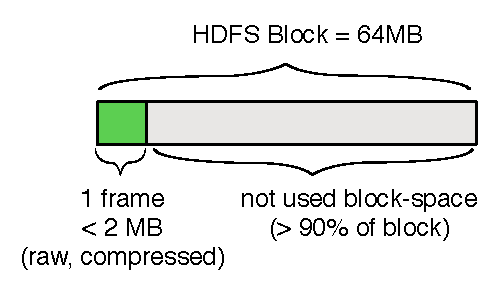
\includegraphics[scale=0.9]{diagrams/no-sequence-file.pdf}
  \caption{When storing a small file in HDFS, it still takes up an entire block. The grey space is not wasted on disk, but causes the \textit{name-node} memory problems.}
  \label{fig:no-sequence-file}
\end{figure}

The problem stemming from writing small files manifests not directly by impacting the used disk space, but in increasing memory usage in the clusters so called \textit{name-node}. The name-node is responsible for acting as a lookup table for locating the blocks in the cluster. Since name-node has to keep 150KB of metadata for each block in the cluster, creating more blocks than we actually need quickly forces the name-node to use so much memory, that it may run into long garbage collection pauses, degrading the entire cluster's performance. To put precise numbers to this -- if we would be able to store 500MB of data in an optimal way, storing them on HDFS would use 8 blocks -- causing the name node to use approximately 1KB of metadata. On the other hand, storing this data in chunks of 2MB (for example by storing each frame of a movie, uncompressed) would use up 250 HDFS blocks, which results in additional 36KB of memory used on the name-node, which is 4.5 times as much (28KB more) as with optimally storing the data! Since we are talking about hundreds of thousands of files, such waste causes a tremendous unneeded load on the name-node.

It should be also noted, that when running map-reduce jobs, Hadoop will by default start one map task for each block it's processing in the given Job. Spinning up a task is an expensive process, so this too is a cause for performance degradation, since having small files causes more \textit{Map tasks} being issued for the same amount of actual data Hadoop will spend more time waiting for tasks to finish starting and collecting data from them than it would have to.

% ------------------------------------------------------------------------------------------------------------------------------------------------
\subsubsection{Sequence Files}
\label{sequence-file}
The solution applied in the implemented system to resolve the small files problem is based on a technique called ''Sequence Files'', which are a manually controlled layer of abstraction on top of HDFS blocks. There are multiple Sequence file formats accepted by the common utilities that Hadoop provides \cite{hadoop-seq-files} but they all are \textit{binary header-prefixed key-value formats}, as visualised Figure \ref{fig:sequence-file}.


\begin{figure}[ch!]
  \centering
  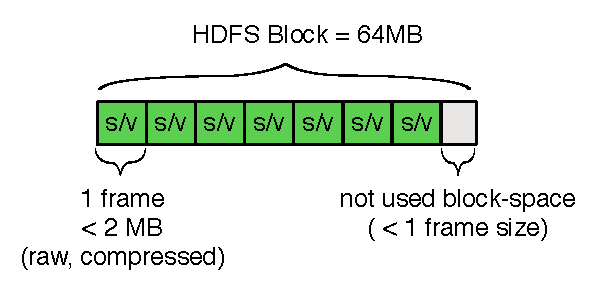
\includegraphics[scale=0.9]{diagrams/sequence-file.pdf}
  \caption{A SequenceFile allows storing of multiple small chunks of data in one HDFS Block.}
  \label{fig:sequence-file}
\end{figure}

Using Sequence Files resolves all previously described problems related to small files on top of HDFS. Files are no longer ''small'', at least in Hadoop's perception,
since access of frames of a movie is most often bound to access other frames of this movie we don't suffer any drawbacks from such storage format.

Another solution that could have been applied here is the use of HBase and it's key-value design instead of the explicit use of Sequence Files, yet this would not yield much performance nor storage benefits as HBase stores it's Table data in a very similar format as Sequence Files. The one benefit from using HBase in order to avoid the small files problem would have been random access to any frame, not to ''frames of this movie'', but since I don't have such access patterns and it would complicate the design of the system I decided to use Sequence Files instead.



% ------------------------------------------------------------------------------------------------------------------------------------------------
\subsection{Tuning replication factors}
\label{sec:tuning-replication-factors}

One of the many tuneable aspects of Hadoop deployments that can have a very high impact on the clusters performance is the \textit{replication factor}.

\begin{figure}
  \centering
  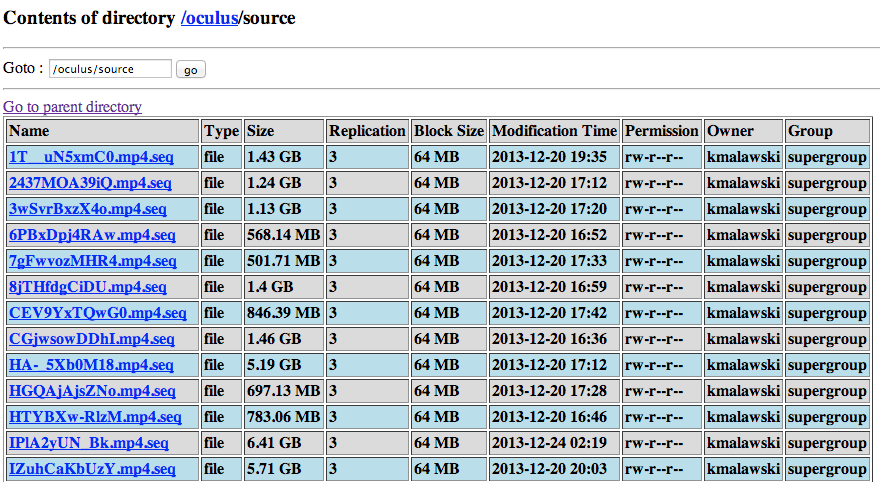
\includegraphics[width=\textwidth]{img/hadoop/hdfs_show-replication}
  \label{fig:hdfs-replication-factors}
  \caption{HDFS on-line browser, running on datanode (port: 50075)}
\end{figure}

\subsection{Tuning number of nodes}
\label{sec:tuning-number-of-nodes}



% ------------------------------------------------------------------------------------------------------------------------------------------------
\section{Scaling the Loader (actor system)}
\label{sec:scaling-akka}

\todo{scale it to more nodes...}
